	\chapter{宇宙的结构}
\indent

   在20世纪前半页, 爱因斯坦(Einstein)描述了时间与空间的原理, 与此同时, 尼尔斯·波尔(Niels Bohr)和他年轻的学徒醉心于描述物质的奇异的量子现象的方程. 在这个世纪的下半页, 物理学家在这两个理论基础之上, 把这两个全新的理论应用到描述自然现象的各个领域: 从宇宙的宏观结构到基本粒子的微观结构. 我将在这一章讲述前一个, 在下一张讲述后一个。

   这章主要由简单的草图组成. 这样的原因是在实验, 测量, 数学以及严密的推理之前, 科学最首要的是关于图像. 科学从图像开始. 科学思维是由从同以往不同的角度"看待"事物的能力培养出的. 我想在这里提供一个在不同看法间旅程的简要的, 适度的轮廓.
		
	\bc
	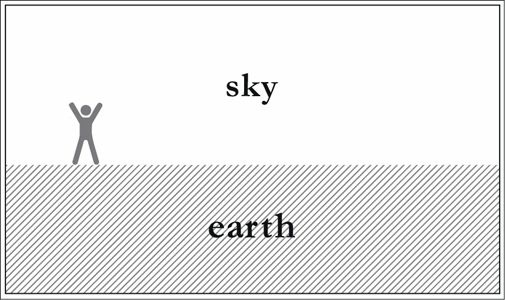
\includegraphics[width=.9\textwidth]{img/31.jpg}\\[12pt]
	\ec

   上面这张图代表了宇宙在数千年之间是如何被理解的: 土地在下面,天空在上面. 阿那克西曼德(Anaximander)在26个世纪之前完成了第一次伟大的科学革命, 他把上面的宇宙的图景换成了下面的样子,那时他正在试图弄清楚太阳, 月亮和星星是如何绕着我们旋转的.

	\bc
	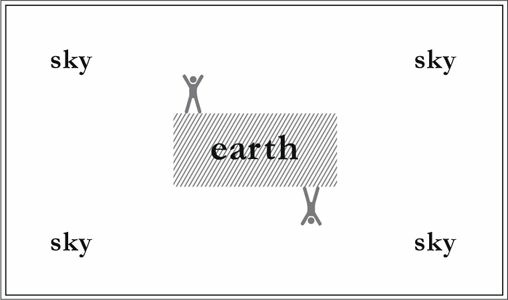
\includegraphics[width=.9\textwidth]{img/32.jpg}\\[12pt]
	\ec

   现在天空环绕在地球的四周, 而不仅仅是它的上方, 地球是悬挂在太空中的巨石, 没有落下. 很快有人(也许是帕门尼斯(Parmenides),也许毕达哥拉斯(Pythagoras))意识到, 球形是这个悬空的地球的最合理的形状, 因为其所有方向都是相同的, 亚里士多德(Aristotle)设计了令人信服的科学论证, 以证实地球和环绕地球四周的各种天体在其中运行的天空球形本质. 这是最后得到的宇宙的图像.

	\bc
	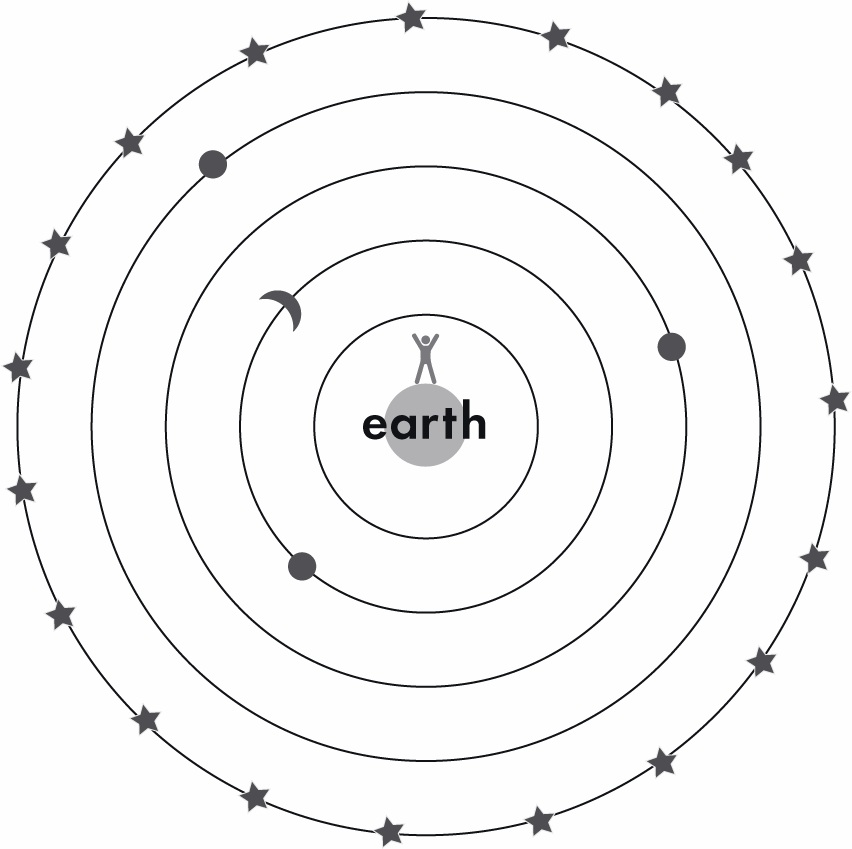
\includegraphics[width=.9\textwidth]{img/33.jpg}\\[12pt]
	\ec

   这个宇宙, 如亚里士多德(Aristotle)在他的作品"论天"中所描述的那样, 是世界的图像, 直到中世纪的结束, 它仍然是地中海文明的特征. 这是丹特(Dante)和莎士比亚(Shakespeare)在学校学习的世界的图像. 

   哥白尼(Copernicus)的下一次飞跃,开创了所谓的伟大的科学革命。哥白尼(Copernicus)的世界与亚里士多德(Aristotle)的世界并没有很大的不同.

	\bc
	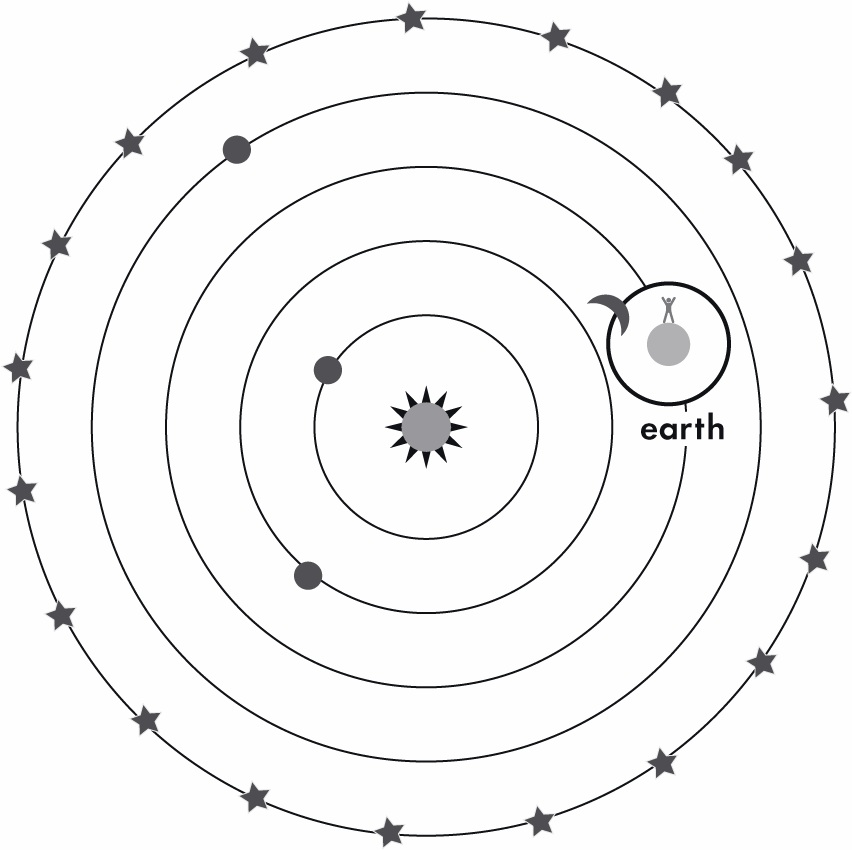
\includegraphics[width=.9\textwidth]{img/34.jpg}\\[12pt]
	\ec

   但是实际上有一个重要的区别。吸取了在古代就已经被考虑过的想法之后,哥白尼(Copernicus)了解到并且表明我们的地球不是行星舞会的中心,而是太阳在那里。我们的星球成为其中之一,高速地绕地轴和太阳的运转。

   我们认知的增长从未停止, 随着仪器的改良我们很快认识到我们的太阳系不过是其他众多太阳系的其中一个, 并且我们的太阳不过是一颗与其他恒星差不多的恒星. 一粒极微小的尘埃在一团由一千亿颗星星组成的磅礴星云---银河系之中。

	\bc
	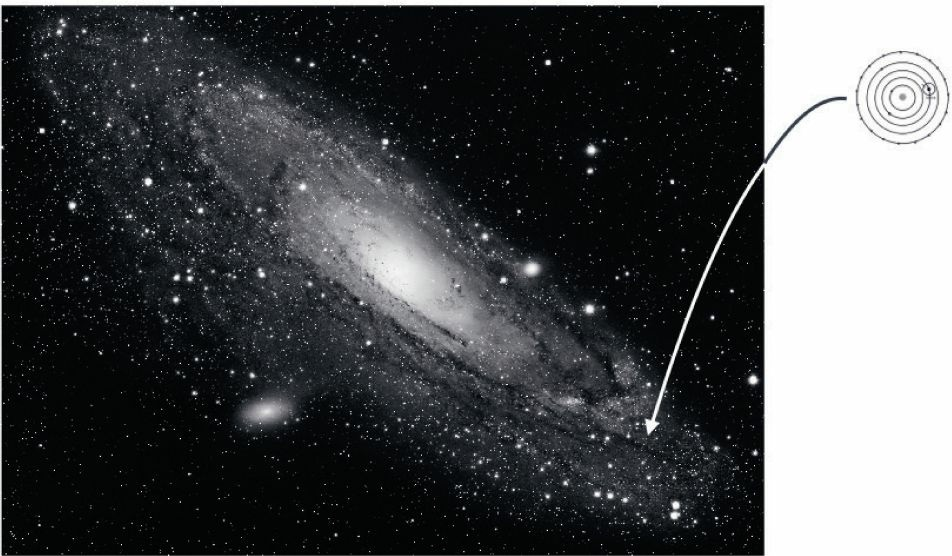
\includegraphics[width=.9\textwidth]{img/35.jpg}\\[12pt]
	\ec

   然而, 那些研究星云, 也就是群星之间发白的云状物, 的天文学家十九世纪三十年代所做出的精确测量表明, 我们的银河系也不过是, 由无数星系组成的绵延到人类最先进的望远镜所能观测到的最远处星空的巨大星系团中的沧海一粟. 人类的宇宙图景始终如一, 毫不停歇地扩张着. 

   以下插图并非是一副画, 它是哈勃太空望远镜拍摄的一副照片. 这张照片展现了一副比以往我们用最强大的望远镜所能看到的还要深的太空图景---如果用肉眼去观测, 这不过是黑色天空中极小的一块碎片. 透过哈勃太空望远镜 一片极其遥远的星尘展现在眼前. 图中每一个黑色的点都是一个包含了上千亿颗像我们的太阳这样的恒星的星系. 而在近几年的观测中, 我们发现这些恒星中的大部分都有行星绕其左右. 正因如此, 宇宙中应当有数千万亿亿的地球这样的行星. 而且这总发生在我们观测的任一方向上.

	\bc
	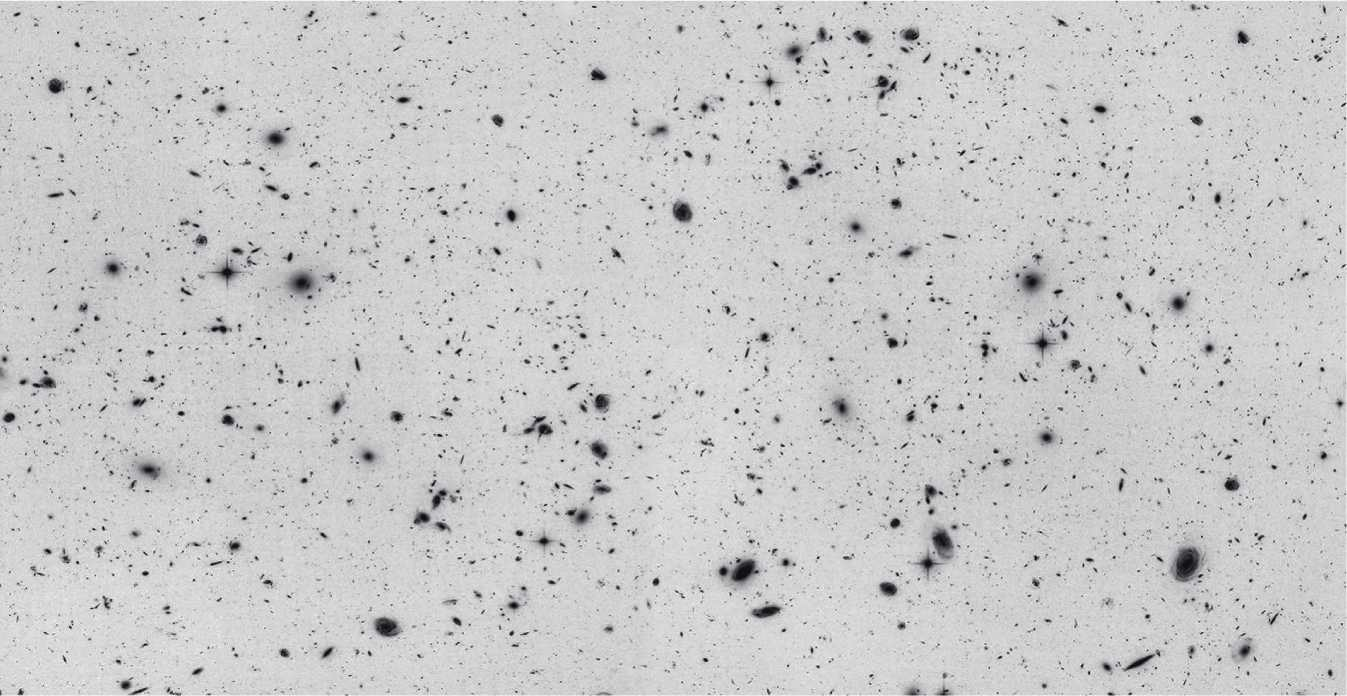
\includegraphics[width=.9\textwidth]{img/36.jpg}\\[12pt]
	\ec	
	\bc
	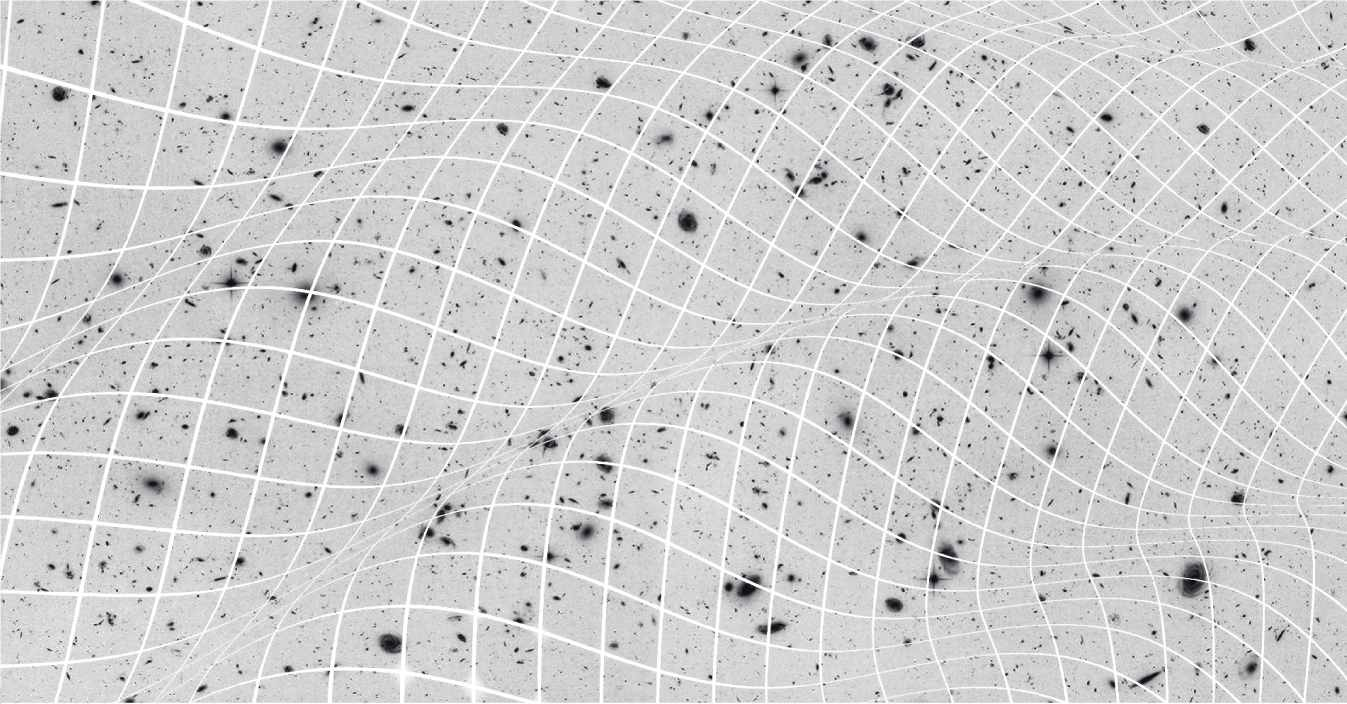
\includegraphics[width=.9\textwidth]{img/37.jpg}\\[12pt]
	\ec
	\bc
	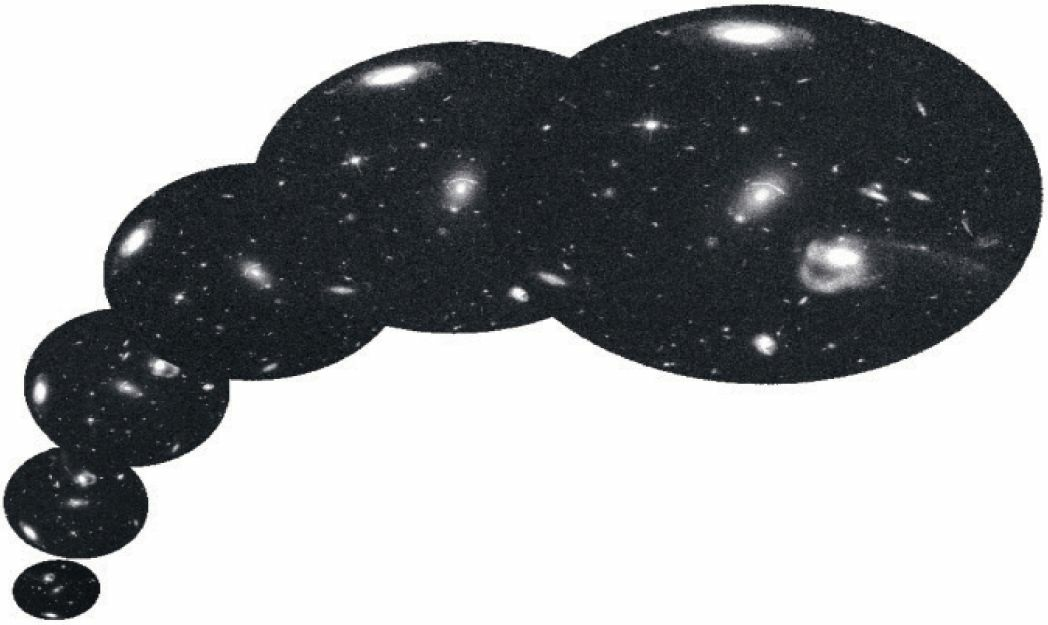
\includegraphics[width=.9\textwidth]{img/38.jpg}\\[12pt]
	\ec

\noindent
